% Doc Setup
\documentclass[11pt]{article}
\usepackage{setspace} 
\doublespacing
\usepackage{amsmath}
\usepackage{graphicx} % Required for inserting images
\usepackage{titlesec} % For custom section titles
\usepackage{lipsum}
\usepackage{hyperref}
\usepackage{float}
\usepackage{mathptmx} % Times New Roman
\usepackage{booktabs}
\usepackage{subcaption}


\usepackage[letterpaper,top=1in,bottom=1in,left=1in,right=1in,marginparwidth=1.75cm]{geometry}


\title{STA 137 Final Project}
\author{Ryan Chiang, Manik Sethi, Muhammad Laiq }
\date{June 2025}
\usepackage{listings}
\begin{document}

\maketitle


\begin{figure}[H]
    \centering
    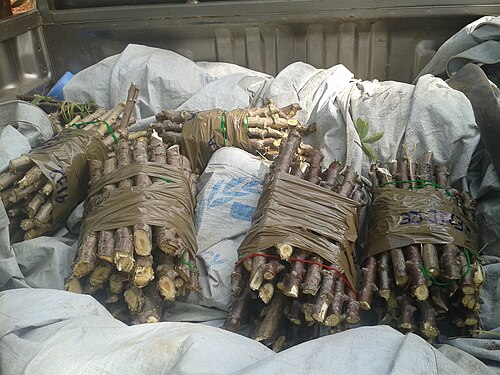
\includegraphics[width=0.3\linewidth]{central_africa_republic.jpg}
    \caption{Central African Lumber}
    \label{fig:enter-label}
\end{figure}




\tableofcontents

%Command for sectioning parts
\newcommand{\numberedpart}[1]{%
    \part{#1}%
}

\section{Introduction}

Agriculture is a vital part of the Central Africa Republic's (CAR) economy, occupying nearly four-fifths of the national work force (Ref 1). Goods such as crops, timber and diamons are essential, and the hallmark of CAR's economy. However, it is rare that these goods stay within the republic itself. Many of these items make their way out of the country as exports, which in turn provide capital to keep the country running.
Studying the trends of GDP and Exports over time allows us to be informed when deciding whether or not the Central African Republic should agree to certain trade deals. By knowing how dependent CAR is on the wealth of other countries, a delicate balance between domestic independence and international exploitation can be found. Time series analysis will offer insights into year-long trends of the economy.


\section{Explanatory Data Analysis}


\section{Model Selection}
\subsection{Transformation}
\subsection{ACF/PACF}
\subsection{Candidate Models}
\subsection{Final Model}

\section{Forecast}

\section{Conclusion}

\newpage

\section{References}

Reference 1: https://www.britannica.com/place/Central-African-Republic/Economy

\begin{figure}[htbp]
  \centering
  %--------------- First image ---------------
  \begin{subfigure}[b]{0.48\textwidth}
    \centering
    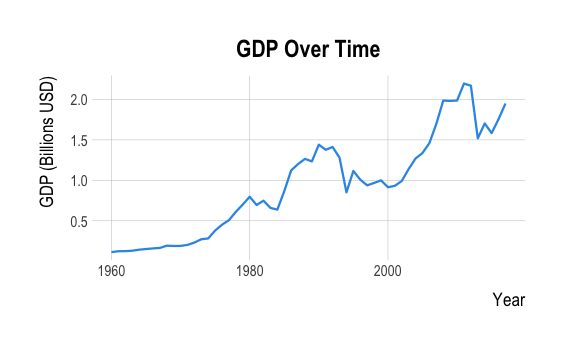
\includegraphics[width=\linewidth]{EDA/GDP_over_Time.png} % replace with your filename
    \caption{Caption for the first image.}
    \label{fig:side:a}
  \end{subfigure}
  \hfill
  %--------------- Second image ---------------
  \begin{subfigure}[b]{0.48\textwidth}
    \centering
    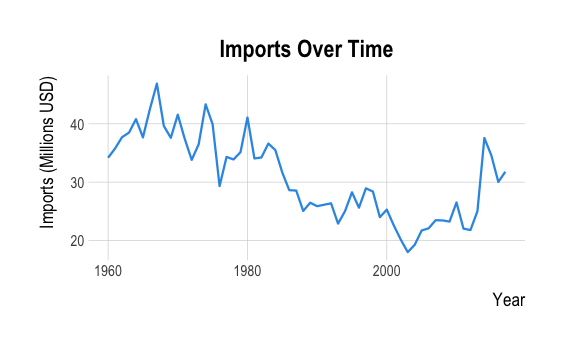
\includegraphics[width=\linewidth]{EDA/Imports_over_Time.png} % replace with your filename
    \caption{Caption for the second image.}
    \label{fig:side:b}
  \end{subfigure}

  \label{fig:side-by-side}

  %--------------- Third image ---------------
  \begin{subfigure}[b]{0.48\textwidth}
    \centering
    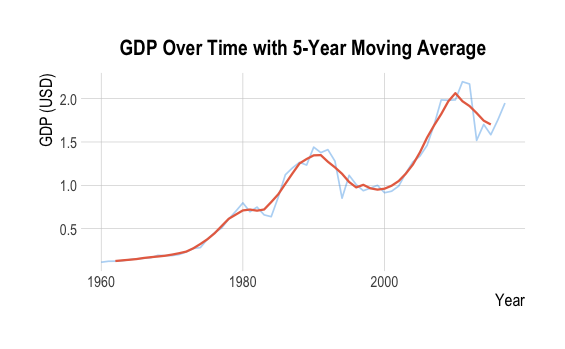
\includegraphics[width=\linewidth]{EDA/GDP_MA5.png} % replace with your filename
    \caption{Caption for the first image.}
    \label{fig:side:a}
  \end{subfigure}
  \hfill
  %--------------- Fourth image ---------------
  \begin{subfigure}[b]{0.48\textwidth}
    \centering
    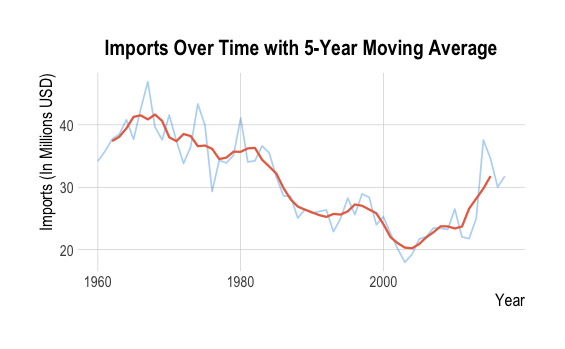
\includegraphics[width=\linewidth]{EDA/Imports_MA5.png} % replace with your filename
    \caption{Caption for the second image.}
    \label{fig:side:b}
  \end{subfigure}
  
  %--------------- First image ---------------
  \begin{subfigure}[b]{0.48\textwidth}
    \centering
    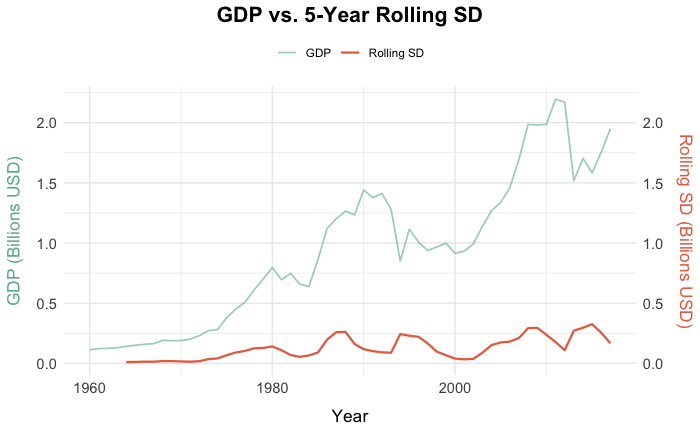
\includegraphics[width=\linewidth]{EDA/GDP_RollingSD5.png} % replace with your filename
    \caption{Caption for the first image.}
    \label{fig:side:a}
  \end{subfigure}
  \hfill
  %--------------- Second image ---------------
  \begin{subfigure}[b]{0.48\textwidth}
    \centering
    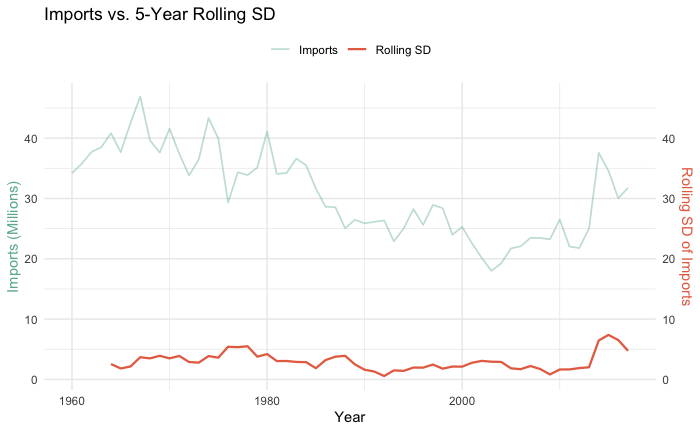
\includegraphics[width=\linewidth]{EDA/Imports_RollingSD5.png} % replace with your filename
    \caption{Caption for the second image.}
    \label{fig:side:b}
  \end{subfigure}

  \label{fig:side-by-side}

  \caption{Graphs for EDA.}
\end{figure}




\end{document}

